\subsubsection{Typ}
En modul som sköter videoinspelning från den främre kameran av testarens ansikte och sparar den till ett givet videoformat.

\subsubsection{Syfte}
Videoinspelning av ansiktet på den som testar applikationen är till för att ge en visuell bild av användaren samt att ytterligare ge information kring hur denna person upplever användargränsnittet på applikationen. Detta betyder att applikationsutvecklaren får mer information för att senare vidareutveckla sin produkt. Komponenter ämnar uppfylla kraven för Kamerainspelning (Se 3.1.3, URD-1).

\subsubsection{Funktionalitet}
Videoinspelning består utav tre stycken klasser; Camera, MediaRecorder samt SurfaceView. Camera är det grundläggande API:t för att kontrollera kamerorna och används både för att ta bilder samt att spela in video. MediaRecorder klassen används för att spela in video från kameran. SurfaceView klassen visar en realtids förhandsvisning av vad kameran ser och visar det på skärmen. Den används alltså för att visa användaren vad kameran spelar in.

\subsubsection{Underordnade komponenter}
Ljudinspelning.

\subsubsection{Beroenden}
Den är inte beroende utav andra komponenter.

\subsubsection{Gränssnitt}
Gränssnittet fungerar så att när denna komponent anropas så startas en Preview för att visa vad som spelas in samt att kameran startar och spelar in film genom MediaRecorder som då producerar en videofil som innehåller video samt ljud från användaren under testet.

\subsubsection{Resurser}
För att kunna spela in med kameran så måste androidenheten först ha en framåtvänd kamera så att det går att spela in användarens ansikte under pågående test. Androidenheten bör också ha en nyare version av Android då alla funktioner kanske inte fungerar ifall enheten har en gammal version installerad.

\subsubsection{Referenser}
Kraven för Kamerainspelningen kan hittas under 3.1.3 i URD-1 men för att få en mer översiktlig insikt i hur kameran fungerar så kan man gå in på länken nedanför för att läsa om Kamera API:et för Androidutveckling.
http://developer.android.com/reference/android/hardware/Camera.html
http://developer.android.com/guide/topics/media/camera.html

\subsubsection{Process}
Det är en ganska avancerad process att starta en videoinspelning och alla delar måste starta i rätt ordning (Detta kan även läsas mer om i länken ovanför).
\begin{enumerate}
\item Öppna kameran för att få ett kamera objekt.
\item Förbered förhandvisning.
\item Starta förhandsvisningen.
\item Starta Videoinspelningen.
	\begin{enumerate}
		\item Lås upp kameran.
		\item Konfigurera MediaRecorder
		\begin{enumerate}
			\item Sätt kameran för videoinspelning, använd kamera objektet.
			\item Bestäm ljudkälla.
			\item Bestäm videokälla.
			\item Bestäm videoformat och kodning.
			\begin{enumerate}
				\item Bestäm videoformat.
				\item Bestäm ljudformat.
				\item Bestäm videokodnings typen.
			\end{enumerate}
			\item Bestäm utgående filformat.
			\item Bestäm förhandsvisnings utformningen för din applikation.
		\end{enumerate}
		\item Förbered MediaRecorder med givna inställningar.
		\item Starta MediaRecorder.
	\end{enumerate}
	\item Stoppa inspelning av video.
	\begin{enumerate}
		\item Stoppa MediaRecorder.
		\item Återställ Mediarecorder (valfri).
		\item Släpp lös MediaRecorder.
		\item Lås Kameran.
	\end{enumerate}
	\item Stoppa förhandsvisningen.
	\item Släpp lös kameran.
\end{enumerate}
Detta är hela förhandlingsloppet för att spela in en video med Camera, MediaRecorder och SurfaceView klasserna i Android. Detta kan man även se nedan i UML diagramet.
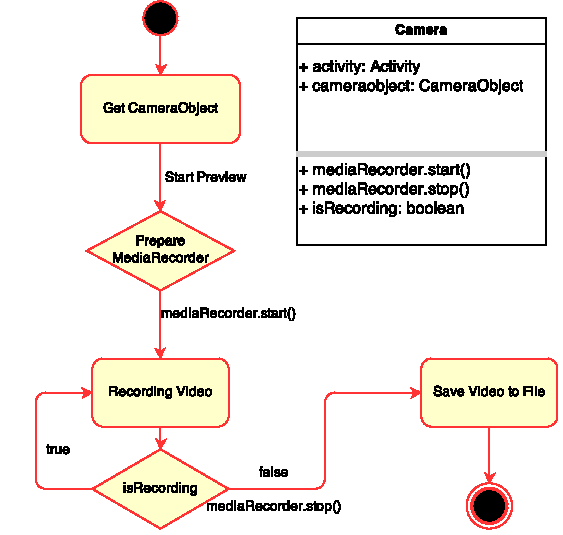
\includegraphics[scale=1.0]{UMLcamera.pdf}

\subsubsection{Data}
Modulen använder sig utav de tre klasserna Camera, MediaRecorder samt SurfaceView. Den behöver alla dessa tre för att skapa en video, dock så sker det mesta i MediaRecorder klassen. Här ges även en sökväg till vart filen ska sparas samt vad videon ska ha för inställningar. Detta styrs till sist genom en boolsk variabel som berättar ifall en video ska spelas in eller inte.
